%%%%%%%%%%%%%%%%%%%%%%%%%
\section{\label{sec:detailed_balance}Metropolis MC acceptance probability and detailed balance}
%%%%%%%%%%%%%%%%%%%%%%%%%

\begin{figure}
\begin{centering}
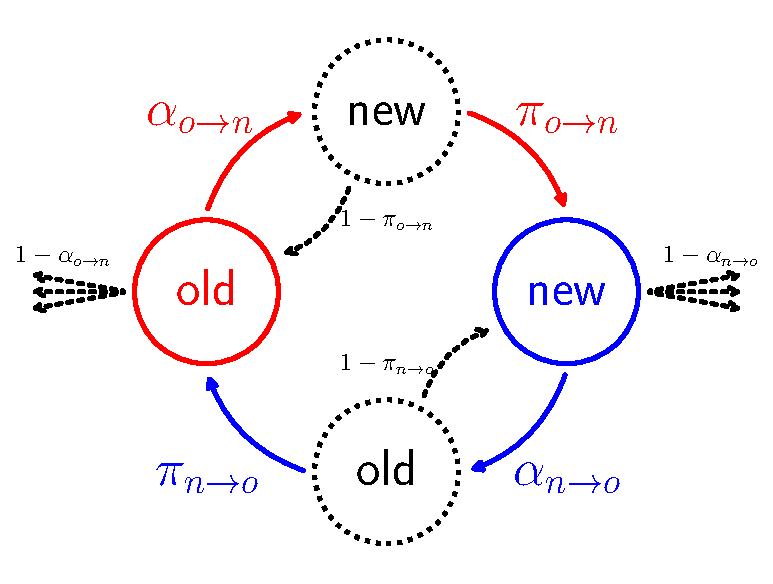
\includegraphics[width=8.5cm]{../figures/detailed_balance.pdf}
\caption{
Probabilities for all possible transitions between two states, old and new, are illustrated.
Proposed configurations and other possible transitions are shown with black dashed circles and arrows, respectively.
Detailed balance is achieved when, for every pair of states, the probability to be in one of the states and then to accept a transition into another state is equal to the probability to be in that other state and then to accept the reverse transition.
}
\label{fig:detailed_balance}
\end{centering}
\end{figure}

In this section, the probability of accepting an attempted MC trial move, or the Metropolis MC trial acceptance probability, denoted by $\chi$, is derived \cite{metropolis_equation_1953, hastings_monte_1970, kofke_monte_1988, allen_computer_1989, frenkel_understanding_2002}.
Ideally, $\chi$ should be close to $1$, so that the trial move in either direction has a high likelihood of being accepted.
The formulation of trial moves is often directed toward this end, while also promoting broader sampling of microstates.

The derivation of $\chi$ in this article requires the condition of detailed balance, shown in Fig.~\ref{fig:detailed_balance}, for a transition from an old microstate, $o$ to a new microstate, $n$,
\begin{equation}
\Pi_o\alpha_{o\rightarrow n}\pi_{o\rightarrow n} = \Pi_n\alpha_{n\rightarrow o}\pi_{n\rightarrow o},
\label{eq:detailed_balance_first}
\end{equation}
where $\Pi_o$ and $\Pi_n$ are the probabilities of being in the old and new microstates, respectively, $\alpha_{o\rightarrow n}$ and $\alpha_{n\rightarrow o}$ are the probabilities of attempting a transition from the old to the new microstate, and vice versa, and $\pi_{o\rightarrow n}$ and $\pi_{n\rightarrow o}$ are the probabilities of accepting those transitions.
Symbols in this article are chosen to follow closely with Ref.~\cite{frenkel_understanding_2002}, but note the different definition of $\pi$.
Detailed balance is a sufficient, but not necessary, condition for ergodic sampling \cite{manousiouthakis_strict_1999}.
For simplicity, we use detailed balance throughout the derivations of this article.
While the microstate probabilities, $\Pi_o$ and $\Pi_n$, are determined solely by the statistical mechanical ensemble, the transition probabilities $\alpha_{o\rightarrow n}$ and $\alpha_{n\rightarrow o}$ depend upon how the MC trial move is implemented.
Thus, Eq.~\ref{eq:detailed_balance_first} provides the route to obtain the trial acceptance probability after the ensemble, trial implementation and acceptance criterion are defined.
Here, \emph{trial implementation} encompasses a great variety of potential moves, such as displacements, volume changes, temperature changes, particle insertions and deletions, alchemical transformations, and more.

In a typical MC simulation, several types of trial moves are employed, with one chosen at random at the beginning of each MC trial.
It is possible that two or more of these trials are capable of producing the same transition between two microstates, albeit in different ways, and with different probabilities.
At first, one might think that the transition probability between two microstates must account for all such ways when determining the acceptance probability $\chi$ to satisfy detailed balance.
Fortunately, this is not the case.
Instead, it is sufficient that each transition method by itself satisfy detailed balance.
It is easy to show that overall detailed balance is satisfied if this ``super-detailed balance" condition is met \cite{frenkel_speed-up_2004}.
In this article, each reversible pair of MC trials is derived as if the pair are the only trials implemented in the simulation.
In special cases, a reversible pair of trials can be obtained by simply repeating the same trial again.
In this special case, the transition probabilities are symmetric.

In general, the Metropolis acceptance criterion is given by,
\begin{equation}
\pi_{o\rightarrow n}=\min(1, \chi),
\end{equation}
where $\chi$ is the Metropolis acceptance probability.
The reverse acceptance probability is $\pi_{n\rightarrow o}=\min(1, 1/\chi)$.
The ratio of $\pi$ is then simplified as,
\begin{equation}
\frac{\pi_{o\rightarrow n}}{\pi_{n\rightarrow o}}=\frac{\min(1, \chi)}{\min(1, 1/\chi)} = \chi,
\label{eq:pi}
\end{equation}
by considering each of the three possibilities, $\chi < 1$, $\chi > 1$ and $\chi=1$, separately.
While the Metropolis acceptance criterion is used throughout this article, other alternatives are possible while maintaining detailed balance.\cite{barker_monte_1965}

Eq.~\ref{eq:detailed_balance_first} may be rearranged to solve for the Metropolis acceptance probability using Eq.~\ref{eq:pi},
\begin{equation}
\chi = \left(\frac{\Pi_n}{\Pi_o}\right)\frac{\alpha_{n\rightarrow o}}{\alpha_{o\rightarrow n}},
\label{eq:detailed_balance}
\end{equation}
where $\chi$ is expressed as the product of two ratios that we refer to throughout this article.

The first ratio in Eq.~\ref{eq:detailed_balance} is the ratio of microstate probabilities, $\Pi_n/\Pi_o$, that may be derived from a given statistical mechanical ensemble, or computed at each step of a converging MC simulation, even if the partition function is not known.
The second ratio may be derived for a given MC trial in a systematic way that is tied very closely to the implementation of the trial.
An important caveat is the ratio $\Pi_n/\Pi_o$ must be expressed in terms of the same set of variables that change during the trial.

